\documentclass[tikz,border=4pt]{standalone}
\usepackage{amsmath}
\begin{document}
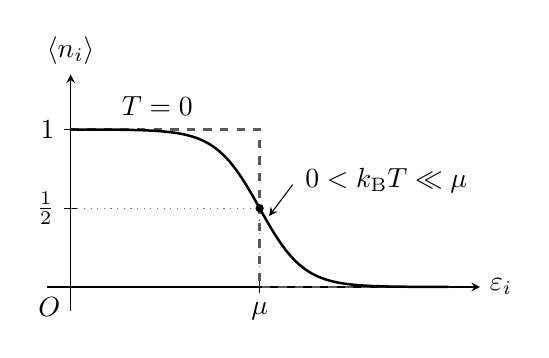
\begin{tikzpicture}[>=stealth, thick, scale=1.0]
  % Axes
  \draw[->, line width=0.4pt] (-0.3, 0) -- (5.2, 0) node[right] {$\varepsilon_i$};
  \draw[->, line width=0.4pt] (0, -0.3) -- (0, 2.7) node[above] {$\langle n_i \rangle$};
  \node[below left] at (0, 0) {$O$};

  % Ticks
  \draw[line width=0.4pt] (0.08, 2.0) -- (-0.08, 2.0) node[left] {$1$};
  \draw[line width=0.4pt] (0.08, 1.0) -- (-0.08, 1.0) node[left] {$\frac{1}{2}$};
  \draw[line width=0.4pt] (2.4, 0.08) -- (2.4, -0.08) node[below] {$\mu$};

  % Guide lines
  \draw[dotted, line width=0.4pt, black!55] (0, 1.0) -- (2.4, 1.0);
  \draw[dotted, line width=0.4pt, black!55] (2.4, 0) -- (2.4, 1.0);

  % T = 0 (dashed step function)
  \draw[dashed, line width=0.9pt, black!65] (0, 2.0) -- (2.4, 2.0) -- (2.4, 0) -- (4.8, 0);

  % 0 < k_B T << mu (solid smooth curve)
  \draw[line width=0.9pt, domain=0:4.8, samples=120]
    plot (\x, {2.0 / (exp((\x - 2.4)/0.28) + 1)});

  % Point at (mu, 1/2)
  \fill (2.4, 1.0) circle (1.5pt);

  % Labels
  \node[above] at (1.1, 2.05) {$T = 0$};
  \node[right] at (2.85, 1.35) {$0 < k_{\mathrm{B}}T \ll \mu$};
  \draw[->, line width=0.4pt] (2.82, 1.3) -- (2.52, 0.9);
\end{tikzpicture}
\end{document}
